\subsection{Development Environment}
\label{subsec:dev_envir}
Die Firmware der Wetterstation wurde im AtmelStudio 7 der Atmel Corp. und der Arduino IDE geschrieben. Die Arduino IDE wurde hauptsächlich verwendet, um notwendige Librarys über dessen \textit{Library Manager} hinzuzufügen. Dies war besonders für die Sensoren BME280 und TSL2561, sowie für die RTC DS3231 und das Schreiben/Lesen der $\mu$SD-Karte notwendig. Anschliessend konnte das gesamte Projekt ins AtmelStudio importiert werden. Grund für diese Importierung ist, dass über AtmelStudio ein ISP (In-System-Programmer) verwendet werden kann. Dies ist mit der Arduino IDE nicht möglich. Der Vorteil bei der Verwendung eines ISP's liegt darin, dass der Mikrocontroller auch nach dem Einbetten in die Hardware programmierbar bleibt. Das Programm wurde in der C/C++ Syntax objektorientiert geschrieben und aufgebaut, somit ist die Firmware der Wetterstation skalierbarer und übersichtlicher.\\

Zur Übersicht der verwendeten Toolchain dient die Tabelle \ref{tab:toolchain}. Zusätzlich sind auch die Downloadlinks der aktuellen Versionen darin enthalten. Die gesamte Toolchain ist als Freeware erhältlich.\\

\begin{table}[h]
\renewcommand{\arraystretch}{1.5}
\centering
\caption{Toolchain}
\label{tab:toolchain}
\begin{tabular}{llp{8cm}}
\toprule 
\textbf{Programm} & \textbf{Version} & \textbf{Link} \\ 
\toprule 
AtmelStudio 7 & 7.0.1645 & \url{https://www.microchip.com/mplab/avr-support/atmel-studio-7} \\ 
\hline 
Arduino IDE & 1.8.5 & \url{https://www.arduino.cc/en/main/software} \\ 
\hline 
PuTTY & 0.71 & \url{https://www.putty.org/} \\ 
\bottomrule 
\end{tabular} 
\end{table}

\subsubsection{In-System-Programmer}
\label{subsubsec:insystemprogrammer}

\begin{minipage}[b][6.5cm][t]{0.5\textwidth}
Als ISP wird der AVR Dragon von Atmel verwendet. Dieser ist ein kostengünstiges Entwicklungstool, welches alle Programmiermodi für die Atmel AVR-Device Familien (z.B. der verwendete atmega2560 Mikrocontroller, siehe \textbf{Referenz}) unterstützt. Er enthält auch eine vollständige Debugging-Unterstützung für die meisten AVR-Devices. Diese wurde aber in diesem Projekt nicht genutzt. Der AVR Dragon wird über das USB 2.0 Kabel (Typ B) gespiesen, mit welchem er an den Computer angeschlossen wird. \cite{avrdragonug}\\

\end{minipage}
\begin{minipage}[b][6.5cm][t]{0.48\textwidth}
\centering
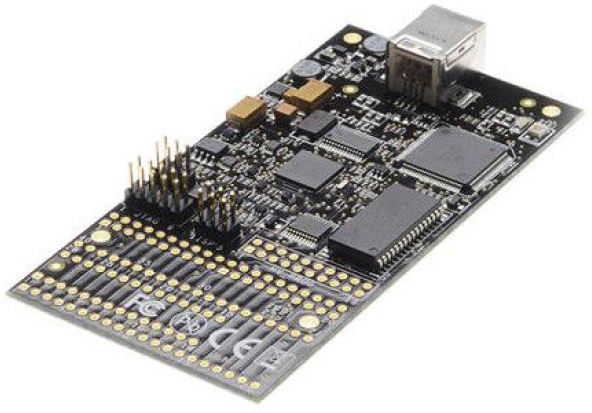
\includegraphics[width=\textwidth]{graphics/ISP/avr_dragon.PNG}
\captionof{figure}{AVR Dragon \cite{avrdragonug}}
\end{minipage}

\paragraph{Programmierinterface}
\label{para:programmierinterface}

Der AVR Dragon kann direkt mit dem Target Board, also der Wetterstation verbunden werden. Dafür werden vom AVR Dragon verschiedene Programmierinterfaces unterstützt: \cite{avrdragonug}\\

\begin{itemize}
	\item SPI Programming 
	\item High Voltage Serial Programming
	\item Parallel Programming
	\item JTAG Programming (\textit{D})
	\item PDI Programming (\textit{D})
	\item aWire Programming (\textit{D})
\end{itemize}
Jene, welche mit einem (\textit{D}) gekennzeichnet sind, dienen auch als Debugging Interface. In Bezug auf das Target Board wird der atmega2560 Mikrocntroller der Wetterstation über das SPI Interface programmiert. Der dafür vorgesehene SPI Header (6-Pin Header) ist auf dem AVR Dragon bereits gemounted, wodurch keine Lötarbeiten erforderlich sind (Abb. \ref{fig:spiheader}, rotes Rechteck).\\

\begin{center}
\begin{minipage}[b][7cm][t]{0.4\textwidth}
\centering
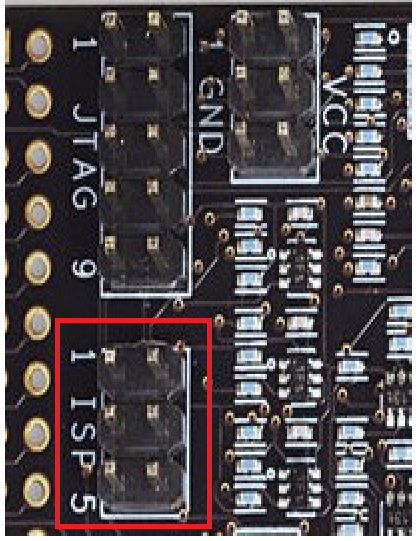
\includegraphics[height=6cm]{graphics/ISP/spi_header.PNG} 
\captionof{figure}{SPI Header \cite{avrdragonug}}
\label{fig:spiheader}
\end{minipage}
\begin{minipage}[b][7cm][t]{0.58\textwidth}
\centering
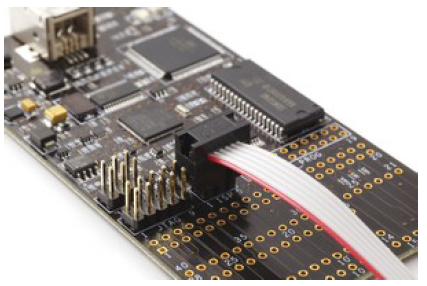
\includegraphics[height=6cm]{graphics/ISP/spi_header_anschluss.PNG} 
\captionof{figure}{Anschluss \cite{avrdragonug}}
\label{fig:spiheader_anschluss}
\end{minipage}
\end{center}

Beim Anschließen des Target Boards sollte darauf geachtet werden, dass die Speisespannung des Targets (3.3V) an dem Pin 2 des Headers angeschlossen ist. Somit kann der AVR Dragon mittels internem Level Converter alle Signale zwischen dem Target Board und sich selbst dem Target anpassen. Das Flachbandkabel sollte also wie in der Abbildung \ref{fig:spiheader_anschluss} angeschlossen werden.

\subparagraph{Zu Beachten:}
Da die $\mu$SD-Karte auf dem Target Board auch über das SPI Interface an den Mikrocontroller angeschlossen ist, so sollten die Jumper beim Anschließen entfernt werden. Es könnte zu Komplikationen führen, wenn Peripherie beim Flash-Vorgang noch an das SPI Interface angeschlossen ist.\\

\paragraph{Device Programming}
\label{para:device_programming}
Um auf das Target (Wetterstation) das Programm flashen zu könenn, müssen noch einige Dinge berücksichtigt werden. In diesem Kapitel wird das wichtigste in Kürze für das Device Programming erklärt. Die folgende Bildabfolge (Abb. \ref:{fig:deviceprogramming} bis \ref{fig:flashing}) soll den Ablauf veranschaulicht erklären und aufzeigen, worauf geachtet werden muss.\\

Als erstes muss das Device Programming über die Menübar \textit{Tools/Device Programming} geöffnet werden (Abb. \ref{fig:deviceprogramming}).\\

\begin{figure}[h]
\centering
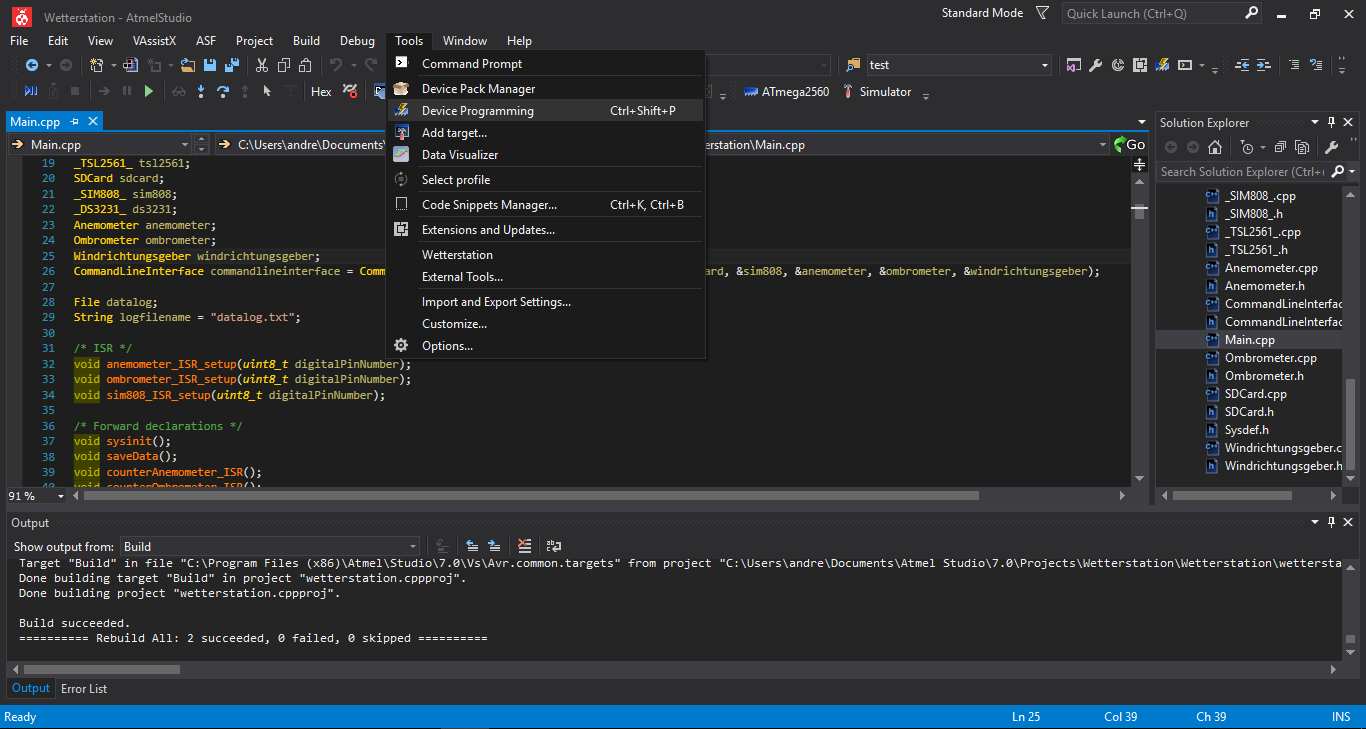
\includegraphics[width=0.7\textwidth]{../../../graphics/device_programming/1.PNG}
\caption{Auswahl Device Programming}
\label{fig:deviceprogramming}
\end{figure}
Wenn der AVR Dragon bereits per USB an den Computer angeschlossen wurde, dann sollte dieser bei Tool (oben links) auswählbar sein. Als Device selbst muss der ATmega2560 gewählt werden. Dies ist vom verwendeten Mikrocontroller abhängig. Das Programmier Interface ist ISP. In der Abbildung \ref{einstellung des ispclocks} ist noch zu sehen, dass der ISP Clock (Flash-Geschwindigkeit) einstellbar ist. Dieser sollte maximal einem Viertel der operierenden Taktfrequenz des Mikrocontrollers sein. In diesem Fall bei 8MHz Taktfrequenz also 2MHz.\\

\begin{figure}[h]
\centering
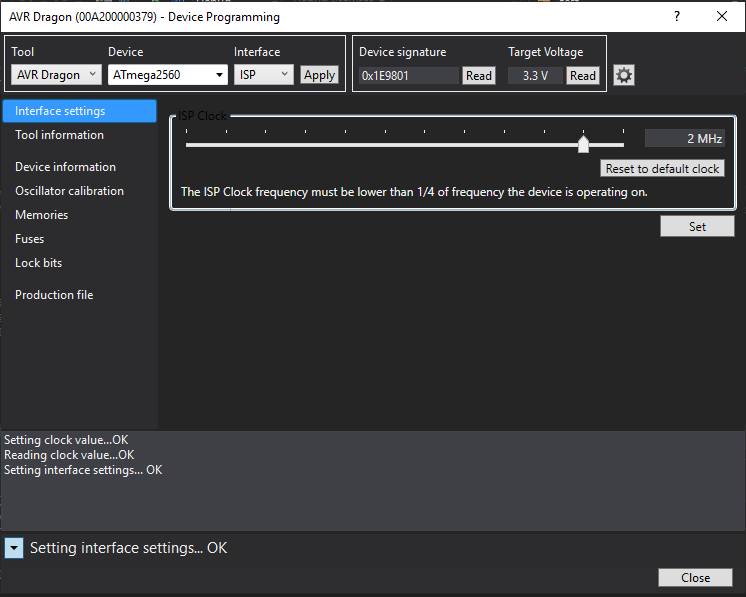
\includegraphics[width=0.7\textwidth]{../../../graphics/device_programming/2.PNG}
\caption{Einstellung des ISP Clocks}
\label{fig:einstellung des ispclocks}
\end{figure}
Für die Fuse Register (Abb. \ref{fig:fuseregister}) ist zu beachten, dass der Clockdivider \textit{LOW.CHKDIV8} abgewählt ist. Beim Kauf des Chips ist dieser oft default mässig eingeschaltet. Da auf dem Target ein externer Oscillator verwendet wird, muss auch dies hier angegeben werden. Dafür das Fuse Register \textit{LOW.SUT_CKSEL} auf einen externen Crystal Oscillator von 3.0 bis 8.0 MHz stellen. Anstatt alle Häckchen einzeln zu setzen, könnten die Values der Fuse Register auch direkt per Hexadezimalzahl angegeben werden. Somit werden alles nötige übernommen. Zum Schluss noch mit \textit{Program} bestätigen. Es können problemlos die Factory Settings überschrieben werden.\\

\begin{figure}[h]
\centering
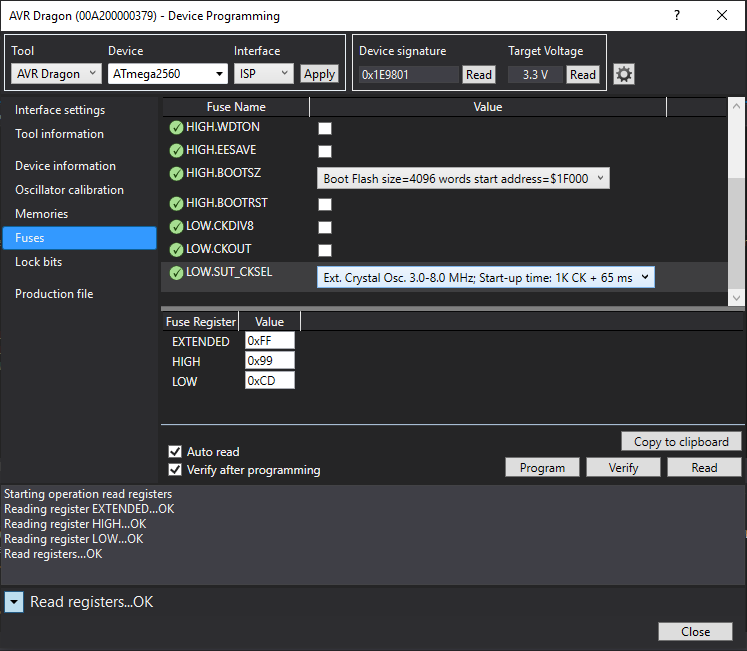
\includegraphics[width=0.7\textwidth]{../../../graphics/device_programming/3.PNG}
\caption{Fuse Register}
\label{fig:fuseregister}
\end{figure}
In der Abb. \ref{fig:lockbits} werden die Lock Bits gezeigt. Hier muss lediglich darauf geachtet werden, dass keine Lock Bits gesetzt werden. Das Lock Bit Register also auf 0xFF einstellen.\\

\begin{figure}[h]
\centering
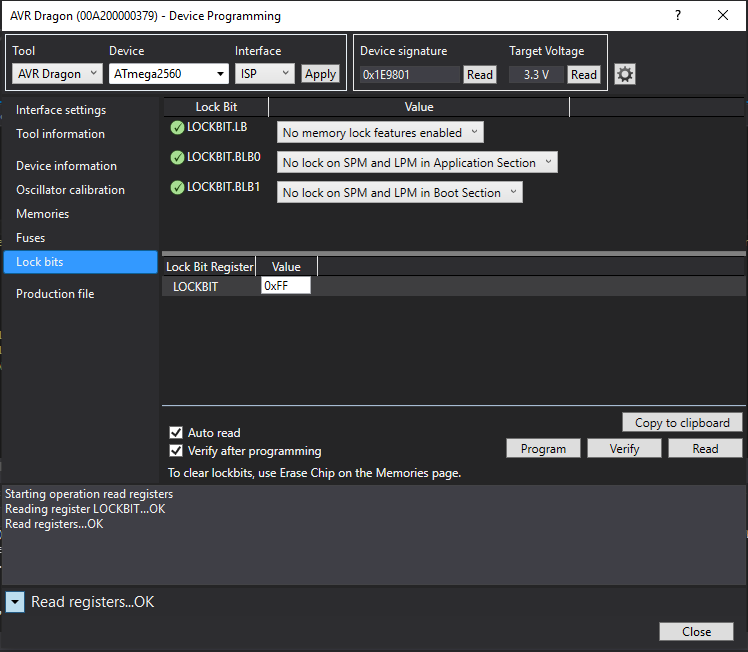
\includegraphics[width=0.7\textwidth]{../../../graphics/device_programming/4.PNG}
\caption{Lock Bits}
\label{fig:lockbits}
\end{figure}
Jetzt kann das geschriebene Programm auf den Mikrocontroller geflashed werden. Von Vorteil ist es, das Häckchen für \textit{Erase device before programming} zu setzen. Ansonsten muss dies jedes mal manuell vor dem Flashen durchgeführt werden. Zum Flashen den Button \textit{Program} drücken.\\

\begin{figure}[h]
\centering
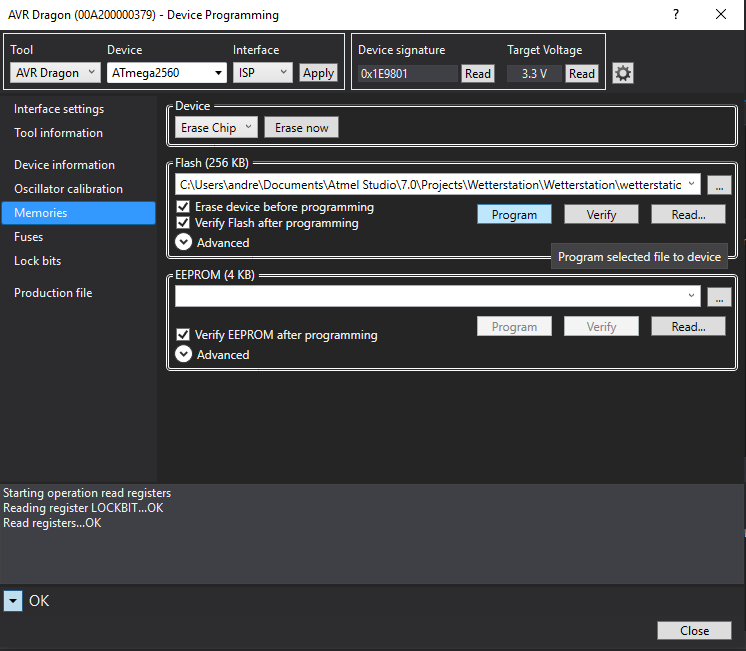
\includegraphics[width=0.7\textwidth]{../../../graphics/device_programming/5.PNG}
\caption{Flashing}
\label{fig:flashing}
\end{figure}
